\chapter{Experiments and Results}
%\section{Experiments}

This chapter describes the following experiments and discusses their
results.
\begin{itemize}
 \item Obtaining good learning parameters for large training sets and
dictionaries.
 %\item Observations of structures of dictionary atoms from different
%groups of images and block sizes.
 \item Convergence of reconstruction quality for different dictionary sizes.
 \item Comparison of reconstruction quality of dictionaries
learned in single and in cluster runs. 
 \item Comparison of compression quality between learned dictionaries, JPEG
and JPEG 2000 on natural images and sketches.
\end{itemize}

\section{Training sets}
\prettyref{sec:learnForTheTask} mentions that one of the key
elements of learning algorithms is learning of specialized
dictionaries. Task specific training data is a common way to solve the problem
of finding the right dictionary. 
%Learning for the task comes into account. 
For example dictionaries for de-noising or in-painting are directly learned from
the images that get restored. If the task gets bigger it sounds logical
to increase the size of training data and take a bigger variety of samples to
learn from into account.  We draw training samples from a large database of
1,000,000 natural JPEG images collected from \url{flickr.com}. 
And have a closer look at differences of learned atoms from a smaller specific
set of sketch images in PNG format (\prettyref{fig:database_images}).

%via clustered training with a large image
% These sets include sketches, still images of animations from Disney and
% post-impressionistic images from Vincent van Gogh.  

\begin{figure}[h]
\centering
\subfloat{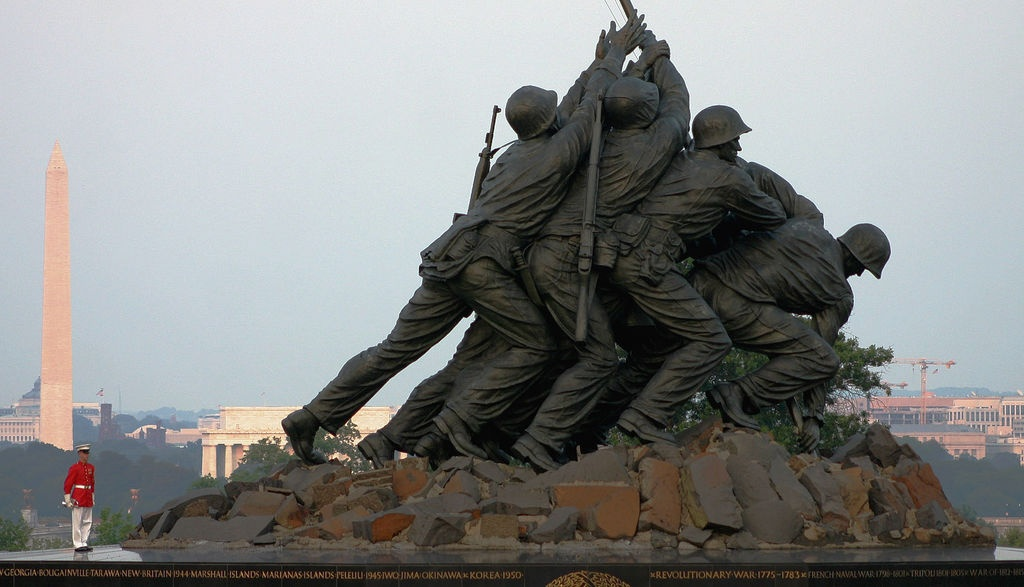
\includegraphics[width = 0.3\textwidth]{images/28979823.jpg}}
\hspace{5mm}
\subfloat{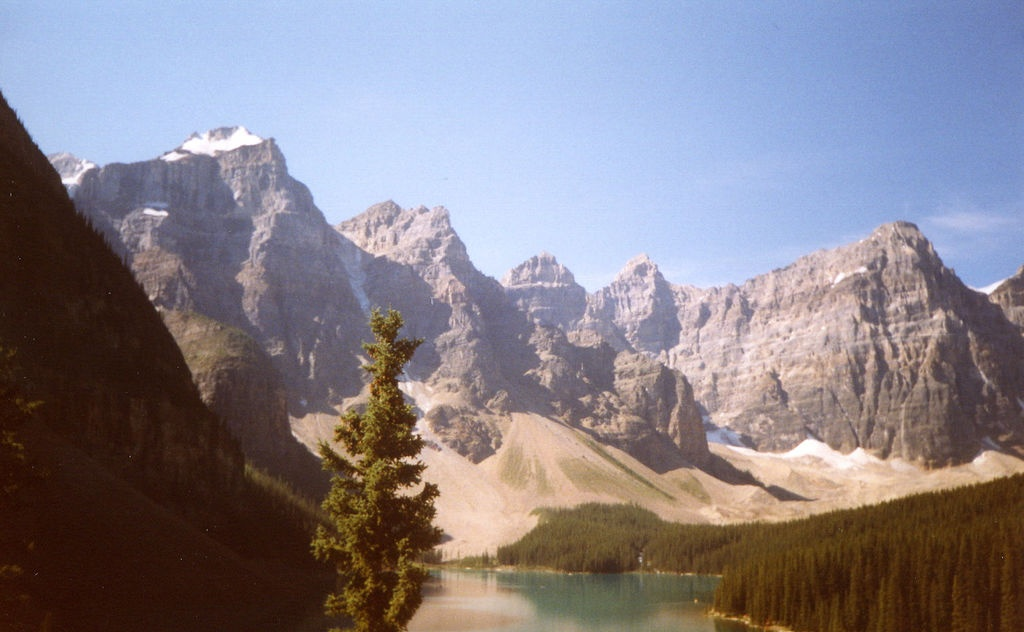
\includegraphics[width = 0.3\textwidth]{images/29018694.jpg}}
\hspace{5mm}
\subfloat{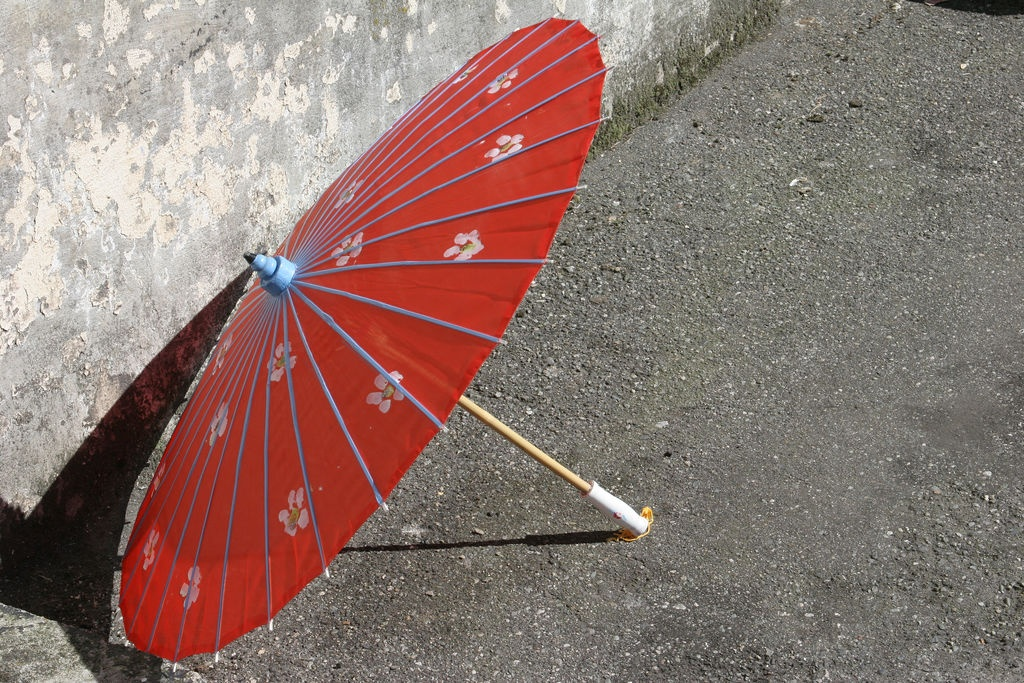
\includegraphics[width = 0.3\textwidth]{images/28874882.jpg}}
\hspace{5mm}
\subfloat{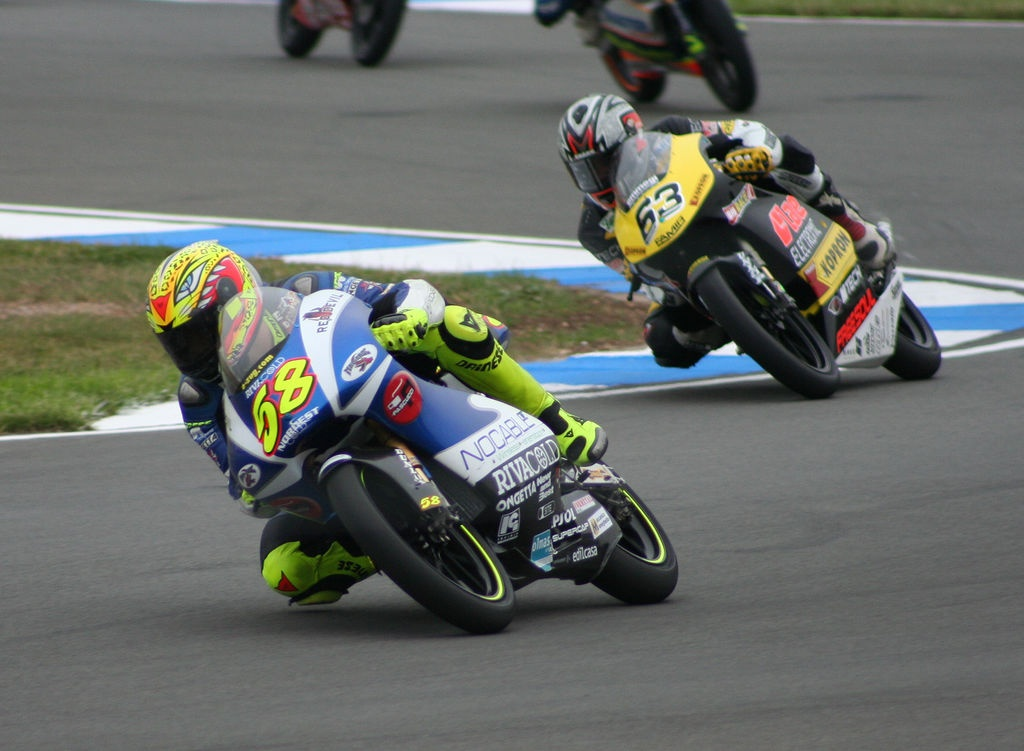
\includegraphics[width = 0.3\textwidth]{images/28803842.jpg}}
\hspace{5mm}
\subfloat{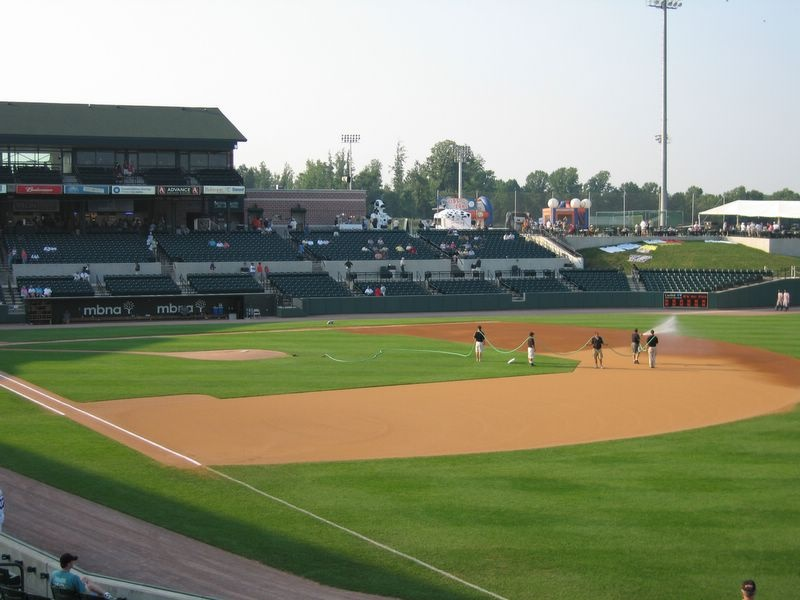
\includegraphics[width = 0.3\textwidth]{images/28894495.jpg}}
\hspace{5mm}
\subfloat{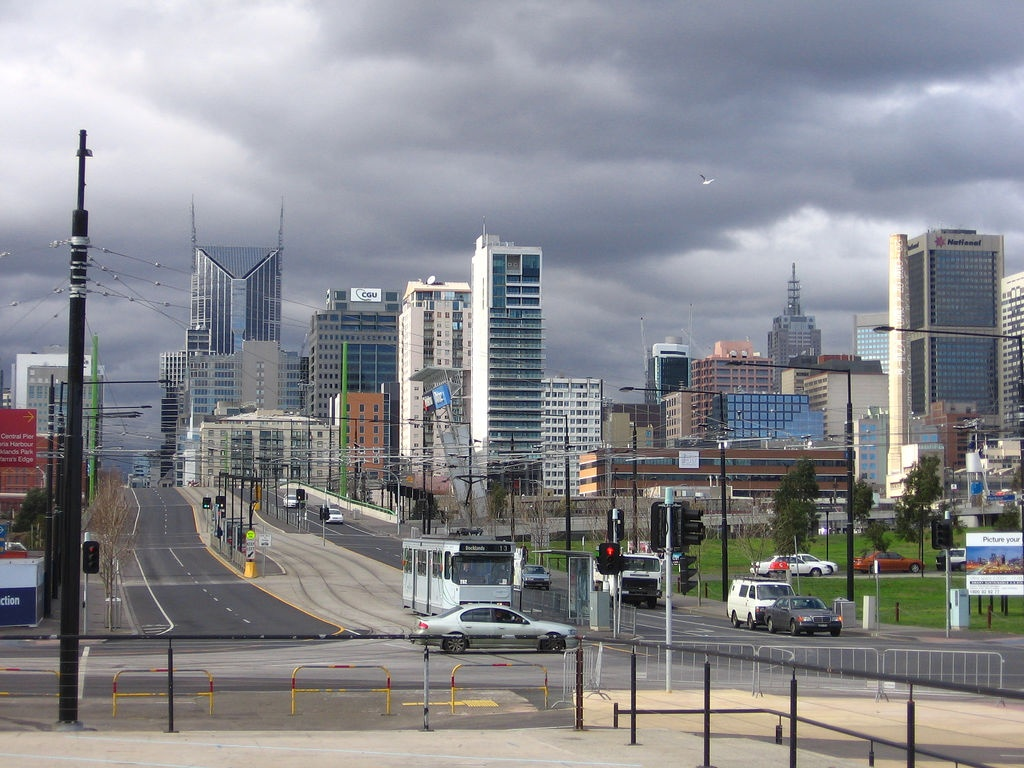
\includegraphics[width = 0.3\textwidth]{images/28952841.jpg}}
\hspace{5mm}
\subfloat{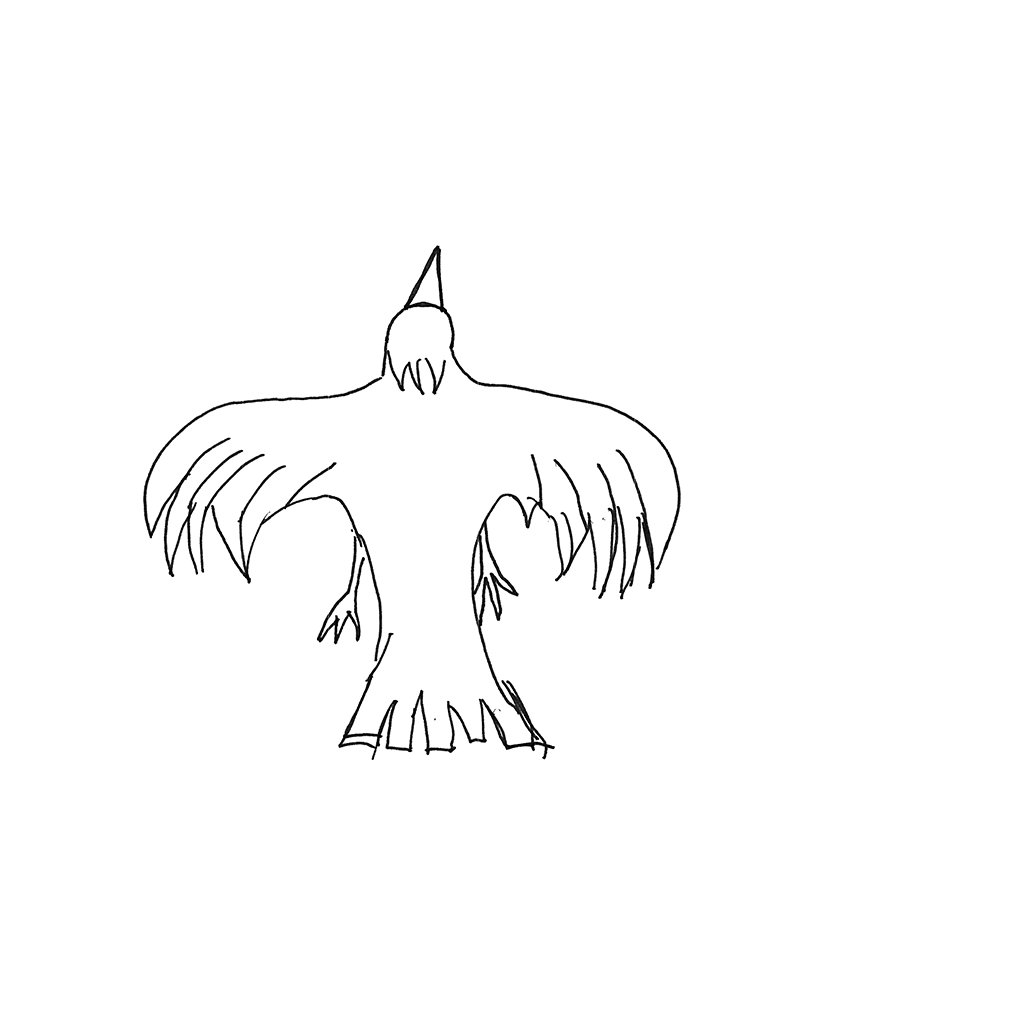
\includegraphics[width = 0.3\textwidth]{images/sketch1.jpg}}
\hspace{5mm}
\subfloat{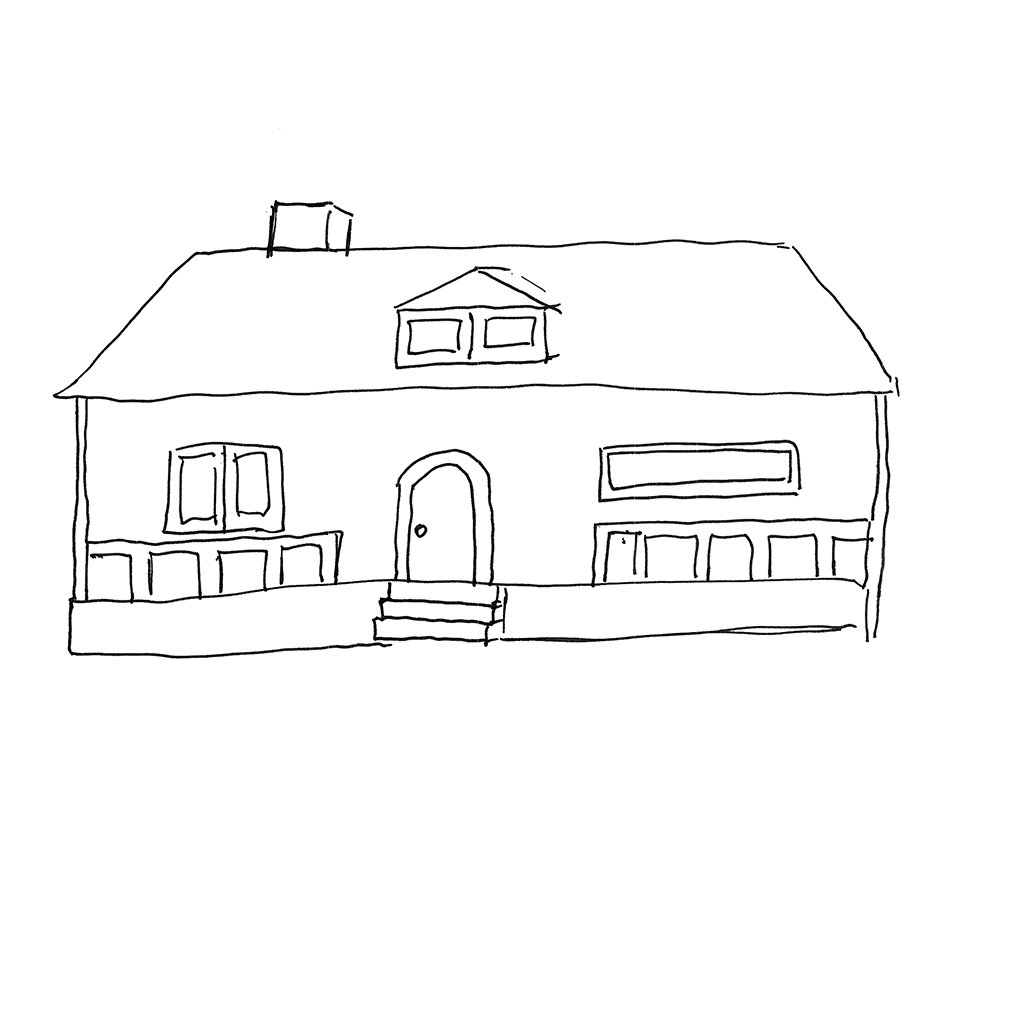
\includegraphics[width = 0.3\textwidth]{images/sketch2.jpg}}
\hspace{5mm}
\subfloat{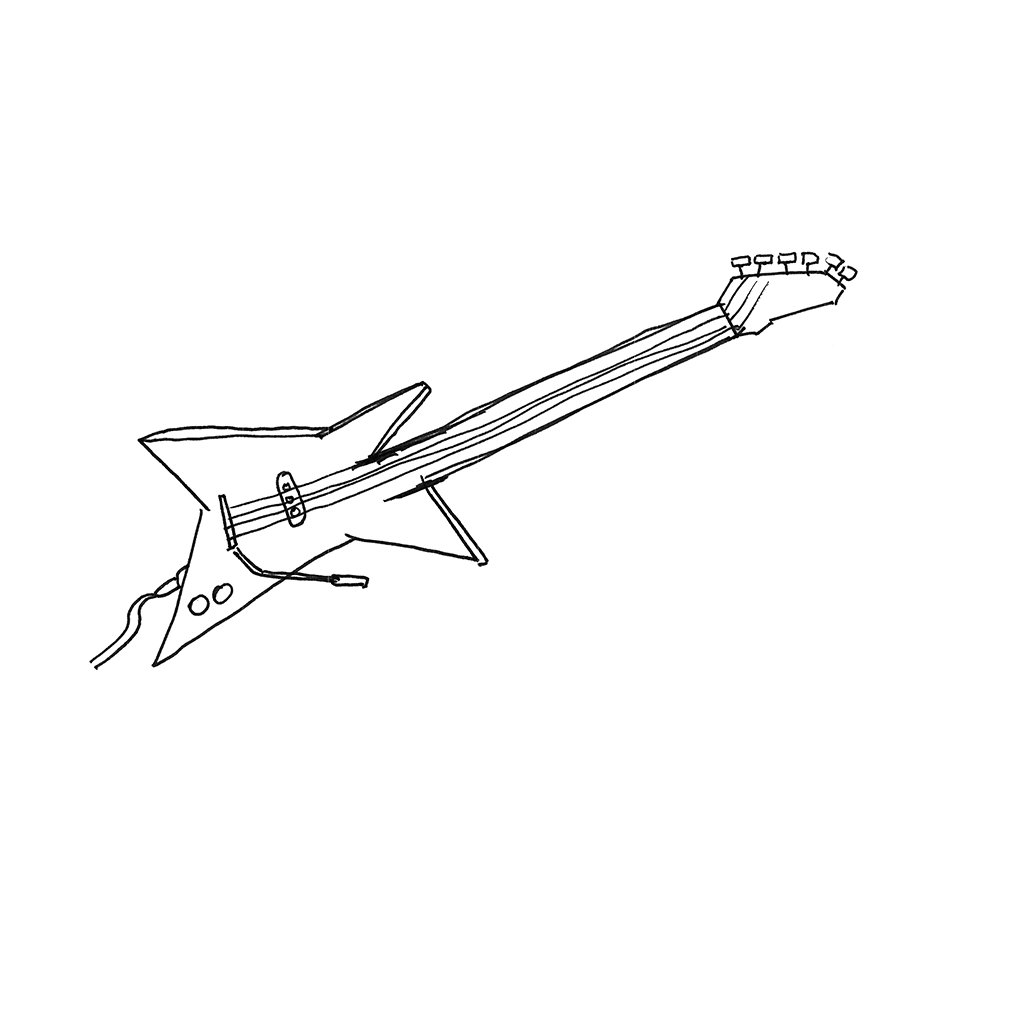
\includegraphics[width = 0.3\textwidth]{images/sketch3.jpg}}
\hspace{5mm}
\caption{example images of natural image and sketch training sets}
\label{fig:database_images}
\end{figure}

\section{Performance measurement}
Before we go further and present the experiments and results it is necessary to
introduce some additional terms. Such as metrics to measure their performance.

\paragraph{Mean squared error (MSE)}  An error measurement that
describes the error between a given or measured reference signal $\vec{x}$
and the reconstruction $\vec{\tilde{x}}$ of it. Mathematically it is defined as
the average of the squared error between two signals.
%The mean squared error is defined as:
\begin{equation*}
 MSE = \frac{1}{n} \sum_{i=0}^{n} \left( {\lVert x_i -
\tilde{x}_i\rVert^{2}}\right)
\end{equation*}
%We primarily use it for testing dictionary learning convergence and as a
%sub term for the measurement described in the next paragraph.

\paragraph{Peak signal-to-noise ratio (PSNR)} Describes the ratio between the
noise affecting a signal and the maximum possible signal amplitude. It is
expressed in a logarithmic decibel scale and undefined for zero
noise.
\begin{equation*}
 PSNR = 20 \cdot \log_{10} \left(\frac{MAX}{\sqrt{MSE}}\right)
\end{equation*}
Where $MAX$ is the maximum possible value of our signal. For an 8-bit
image it would be 255. For a 32-bit normalized image it would be 1.
% $MSE$ is the mean squared error between a reference signal and its
% reconstruction. 

The PSNR is primarily used for comparison of the reconstruction quality of
lossy compression algorithms. Typical values for a lossy reconstruction lie in
a range between 30dB and 
50dB.\footnote{\url{http://en.wikipedia.org/wiki/Peak_signal-to-noise_ratio}}
%e.g. relevant for de-noise

\paragraph{Bits per pixel (bpp)} 
For the comparison of compression ratios of images another well known practice
is to measure the required \emph{bits per pixel} short bpp. The bbp are
calculated by dividing size of the image data by the image's dimensions. For
example an uncompressed RGB color image with 8-bit color depth requires
$24bpp$, respectively a gray scale image with 8-bit for a single
channel requires $8bpp$. Compression algorithms are able to encode
multiple pixels with few coefficient leading to much lower bpp rates.
Looking at other well known compression algorithms such as JPEG or
JPEG 2000 a common ratio is about $\sim1.8bpp$ for average
quality compression (JPEG quality of 50) and less than $\sim1bpp$ for
lower compression.

%\Todo{optinal: example image?, lower bit rates, Lewicki estimate for sparse
%coding}

\paragraph{Test data}
In addition to the introduced metrics it is common practice to use some image
sets to compare test results of the different algorithms and parameter
configurations. As the dictionaries are specifically trained for
reconstruction of data in the training sets
(\prettyref{fig:database_images}). It is mandatory to also use
these images to test the reconstruction and compression quality. 

In addition to this we want to know how good the dictionaries can compress
images outside the database respectively the training set. For
those comparisons we use a selection (\prettyref{fig:USC-SIPI}) from a
well known set of standard test images from the \emph{USC-SIPI Image
Database}\footnote{\url{http://sipi.usc.edu/database/}}. 
%Including pictures such as Lena, Mandrill and Peppers.
\begin{figure}[H]
\centering
%\subfloat{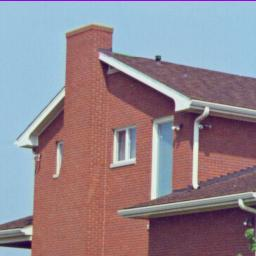
\includegraphics[width = 0.3\textwidth]{images/4_1_05.jpg}}
%\hspace{5mm}
\subfloat{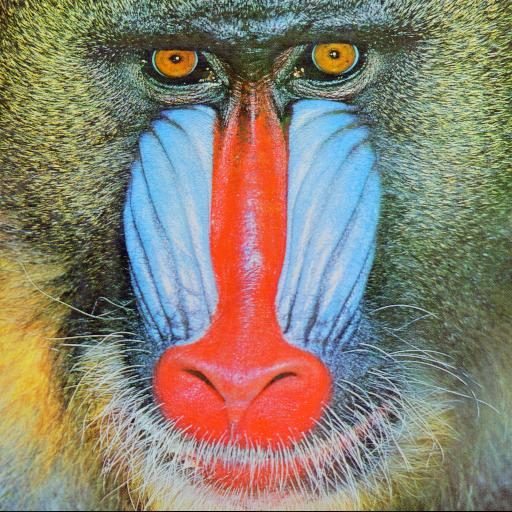
\includegraphics[width = 0.3\textwidth]{images/4_2_03.jpg}}
\hspace{5mm}
\subfloat{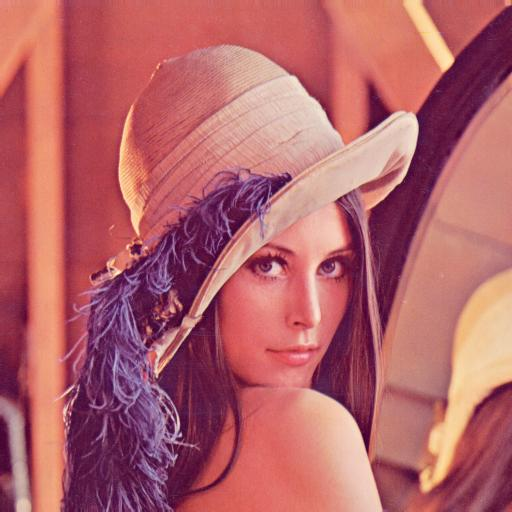
\includegraphics[width = 0.3\textwidth]{images/4_2_04.jpg}}
\hspace{5mm}
%\subfloat{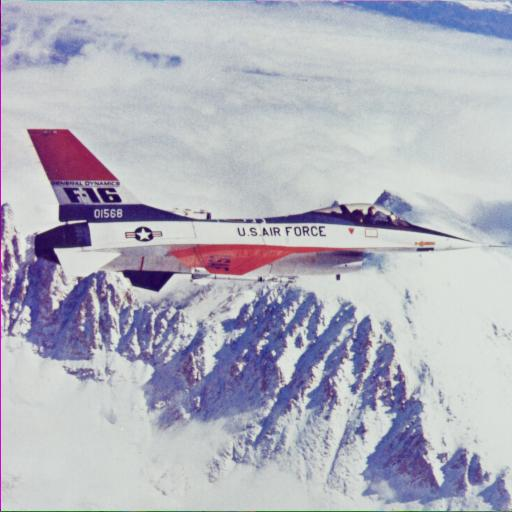
\includegraphics[width = 0.3\textwidth]{images/4_2_05.jpg}}
%\hspace{5mm}
%\subfloat{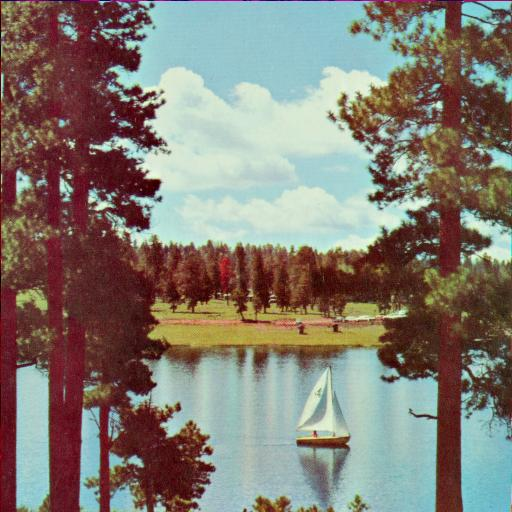
\includegraphics[width = 0.3\textwidth]{images/4_2_06.jpg}}
%\hspace{5mm}
\subfloat{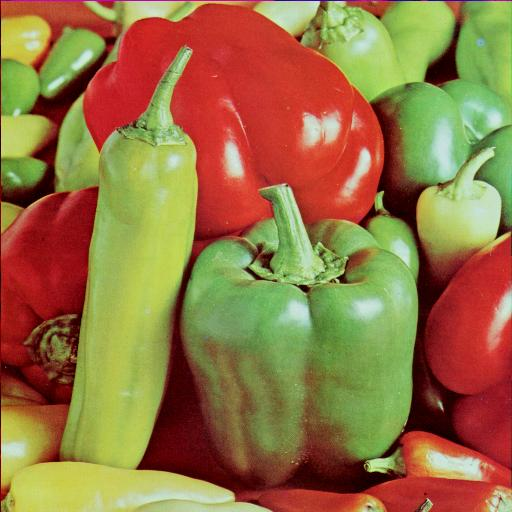
\includegraphics[width = 0.3\textwidth]{images/4_2_07.jpg}}
\caption{test images from USC-SIPI Image Database}
\label{fig:USC-SIPI}
\end{figure}

\section{Hardware setup} 
Computations are made on a cluster of 100 clients. Each 
configured with a AMD Athlon 64 X2 (2x2.6GHz) and 3GB RAM.
The operating system running is Debian Linux with 32-bit kernel. 

\section{Learning parameters}
At first we need to find start parameters for the dictionary learning
algorithm. To experiment with large set of different samples and big
dictionaries. This involves the average number of learning
coefficients, block size, sample selection strategy and mini-batch size.

Mairal et al. already propose some learning parameters for their online
learning algorithm. But as most other they only learn dictionaries with
a small redundancy of up to four times and compact training sets with 100,000
to 1,000,000 samples that get randomly evaluated until convergence of the
dictionary.

We want to find start settings for experiments with large sets of
different samples with no reevaluation of the samples and dictionaries
with much bigger redundancy of 10 to 50 times.

\paragraph{Coefficients}
An average of 10 learning coefficients is suggested as it produces enough
sparseness and leads to good and fast convergence of the dictionaries.
We test if this also applies to big numbers of samples and bigger
dictionaries. We compare the reconstruction quality dependency on the average
number of coefficients in the learning process. 
%The following graphs show the avarage of a set of test images from the training
%set. 
Both OMP (\prettyref{fig:coeffsOMP}) and LARS-Lasso
(\prettyref{fig:coeffsLasso}) runs are made with the following
configuration.
\begin{table}[H]
%\caption{Configuration}
\centering
\begin{tabular}{| c | c | c |}
\hline
\multicolumn{3}{|c|}{configuration}\\
\hline
dict. size & block size & batch size \\
\hline
1024 & $8\times 8$ & 4000  \\
\hline
\end{tabular}
\end{table}

\prettyref{fig:coeffsOMP} and \prettyref{fig:coeffsLasso} show the results for
both algorithms.

\newpage
\begin{figure}[H]
\centering
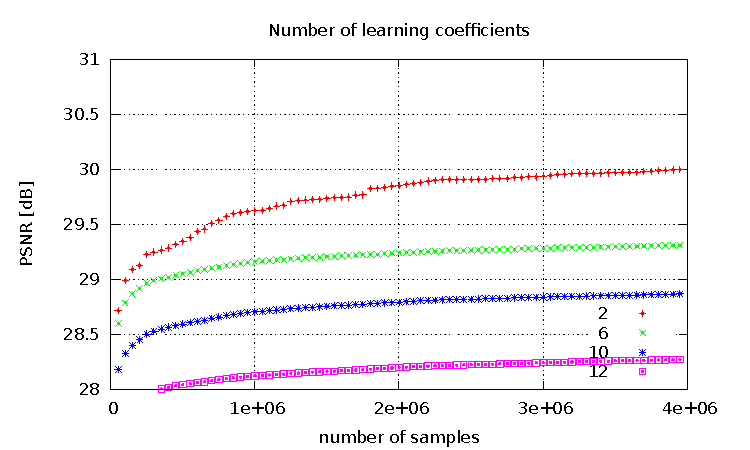
\includegraphics[width =
1.0\textwidth]{../tests/results/coeffsConvergOMP.pdf}
\caption{reconstruction quality for different training coefficients (OMP)}
\label{fig:coeffsOMP}
\end{figure}

\begin{figure}[H]
\centering
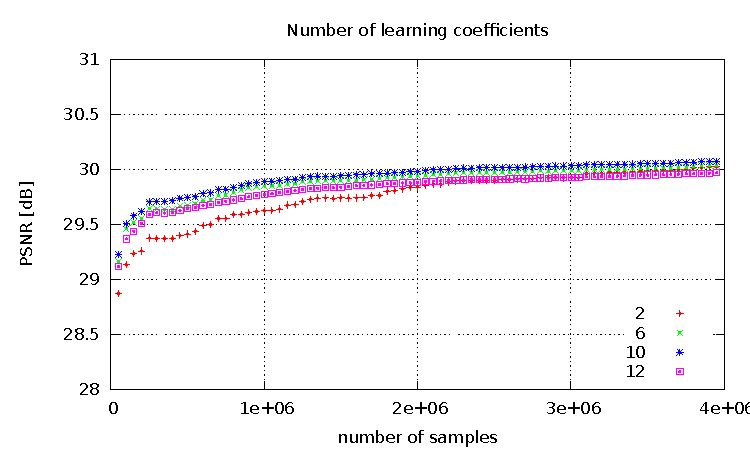
\includegraphics[width = 1.0\textwidth]{../tests/results/coeffsConverg.pdf}
\caption{reconstruction quality for different training coefficients (LARS)}
\label{fig:coeffsLasso}
\end{figure}


% \begin{figure}[H]
% \centering
% \subfloat[2]{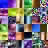
\includegraphics[width =
% 0.2\textwidth]{images/coeffsConvergOMP_0_1.jpg}}
% \hspace{15mm}
% \subfloat[10]{
\includegraphics[width =
% 0.2\textwidth]{images/coeffsConvergOMP_4_1.jpg}}
% \caption{after 50,000 samples}
% \label{fig:coeffsOMP50}
% \end{figure}
% \begin{figure}[H]
% \centering
% \subfloat[2]{
\includegraphics[width =
% 0.2\textwidth]{images/coeffsConvergOMP_0_2.jpg}}
% \hspace{15mm}
% \subfloat[10]{
\includegraphics[width =
% 0.2\textwidth]{images/coeffsConvergOMP_4_2.jpg}}
% \caption{after 2,000,000 samples}
% \label{fig:coeffsOMP2000}
% \end{figure}

% With high number of learning coefficents convergence is reached faster than
% with a low number of coefficents for OMP and LARS-Lasso.
% For larger training sets fewer coefficents can lead to better reconstruction
% quality. 

The first interesting observation is that both algorithms learn good
dictionaries with only a few coefficients. But while the LARS-Lasso is very
constant with different numbers of coefficients the quality of the OMP drops
with increasing number of coefficients. 
Unfortunately using only a few coefficients leads to the problems with big
dictionaries. \prettyref{fig:dictSizeLassoBad} shows a learning process of
LARS-Lasso with about 4 learning coefficients.
\begin{figure}[H]
\centering
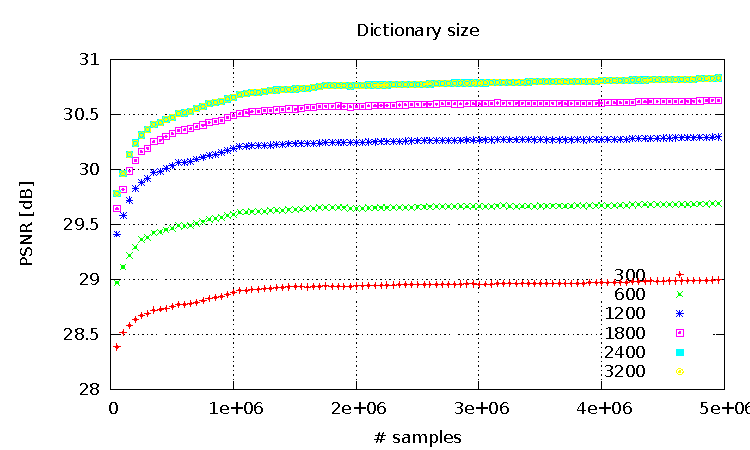
\includegraphics[width = 1.0\textwidth]{../tests/results/dictSizeLasso.pdf}
\caption{reconstruction quality for different dictionary sizes (LARS)}
\label{fig:dictSizeLassoBad}
\end{figure}
Notice two things in this graph. First convergence is almost reached
after 1,000,000 - 2,000,000 training samples. Second even the PSNR is a
logarithmically scale increasing dictionary size reaches a maximum at
about 2,400 atoms. 

The problem is that both algorithms do not learn enough atoms with to few
learning coefficients. Leaving a lot of the dictionary untouched. This can be
addressed with increased number of learning coefficients. But making the OMP
impractical for learning larger dictionaries.
Because of this we concentrated further learning experiments on the LARS-Lasso
with the suggested setting of 10 learning coefficients. 

We also notice that the LARS-Lasso produces dictionaries with better
reconstruction quality than the OMP.

% \begin{figure}[H]
% \centering
% 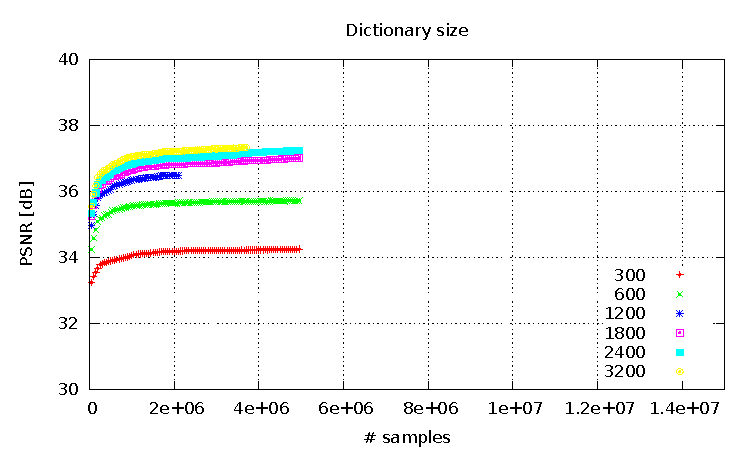
\includegraphics[width = 0.8\textwidth]{../tests/results/dictSizeOMP.pdf}
% \caption{reconstruction quality for different dictionary sizes (OMP)}
% \label{fig:dictSizeSizeOMPBad}
% \end{figure}



\paragraph{Block size}
After the coefficients experiments we compare the reconstruction quality
dependency on block size in the learning process of natural images. 

\prettyref{fig:dict size} shows the results of a dictionary
learning run with block sizes of $n=8,..,20$. The dictionary size for each run
is two times the size of each signal $2m=2n^2$. Coefficients for learning and
reconstruction are adjusted with an average of 2 coefficients for 16 pixels of
the block.

\begin{figure}[h]
\centering
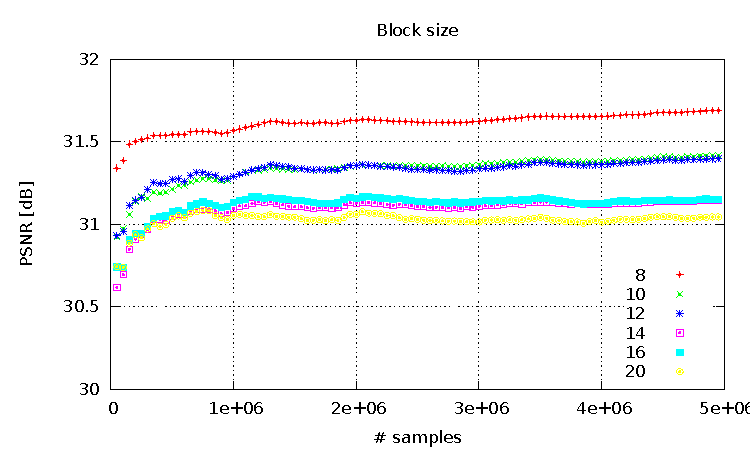
\includegraphics[width =
1.0\textwidth]{../tests/results/blockSizeConverg.pdf}
\caption{reconstruction quality for different block sizes (LARS)}
\label{fig:blockSize}
\end{figure}

While the reconstruction quality decreases slightly with block size. 
The $8\times8$ block size has a significant better reconstruction quality. 
We start to understand why when we have a closer look at the structure of
the atoms. 

\paragraph{Structure}
For the training set from natural JPEG images we tend to learn four major types
of elements (\prettyref{fig:8atoms}).
The ODL algorithm learns atoms similar to combinations of DCT atoms
((a) and (b)). Or similar to wavelet atoms ((c) and (d)).

As our training sets consists of JPEG images it is likely that we actualy learn
the block structure of the JPEG images. This strongly happens when using the
extracting the $8\times 8$ blocks of the JPEG images as samples.
\prettyref{fig:16jpeg_atoms} shows the effect when extracting $16\times 16$
blocks alligned to the JPEG block structure.

When using overlapping samples extraction with no alignment to the JPEG blocks
more wavelet like atoms show up for big block sizes (\prettyref{fig:16atoms})
while the $8\times 8$ do not change significant. 

While looking at this we want to know what structures show samples from other
groups of images. We investigate some atoms of the sketch
dictionary.
The sketch atoms (\prettyref{fig:sketch_atoms}) look way different compared to
the atoms from the natural image set. With a lot of wavelet like atoms. 

We see that both dictionaries primarily capture the structure the underlining
signal provides. 

\begin{figure}[h]
\centering
\subfloat[]{
\includegraphics[width = 0.3\textwidth]{images/gradient.png}}
\hspace{5mm}
\subfloat[]{
\includegraphics[width = 0.3\textwidth]{images/checkerboard.png}}
\hspace{5mm}
\subfloat[]{
\includegraphics[width = 0.3\textwidth]{images/edges.png}}
\hspace{5mm}
\subfloat[]{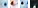
\includegraphics[width = 0.3\textwidth]{images/spot.png}}
\caption{$8\times 8$ atoms of natural images}
\label{fig:8atoms}
\end{figure}
\begin{figure}[h]
\centering
\subfloat{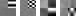
\includegraphics[width = 0.4\textwidth]{images/jpeg_atoms.png}}
\caption{$16\times 16$ of four $8\times 8$ micro blocks}
\label{fig:16jpeg_atoms}
\end{figure}
\begin{figure}[h]
\centering
\subfloat{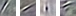
\includegraphics[width = 0.4\textwidth]{images/wavelet.png}}
\caption{$16\times 16$ atoms of natural images}
\label{fig:16atoms}
\end{figure}
\begin{figure}[h]
\centering
\subfloat{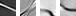
\includegraphics[width = 0.4\textwidth]{images/sketch_atoms.png}}
\caption{$16\times 16$ atoms of sketch images}
\label{fig:sketch_atoms}
\end{figure}


%The learning algorithm can only what the signal provide than the atom from the
%natural image dictionary.

\paragraph{Mini-batch size}
For the small training sets Mairal et al. suggest mini-batch size of two to four
times the size of the the dictionary. No significant observations were made
and we stick to these sizes. 

\clearpage

\section{Dictionary size}
With the right learning parameters to learn from large sets of
different images we want to know how big we can make the dictionaries and
still profit from them. And if reconstruction quality increases with
dictionaries size and when convergence is reached. 

The following configuration is used for the experiments. 
\begin{table}[H]
\centering
\begin{tabular}{| c | c | c |}
\hline
\multicolumn{3}{|c|}{configuration}\\
\hline
coefficients & block size & batch size \\
\hline
10 & $8\times 8$ & 4000  \\
\hline
\end{tabular}
\end{table}

\prettyref{fig:dictSizeGood} does show a different image than
\prettyref{fig:dictSizeLassoBad}. With the right learning parameters 
we better learn bigger dictionaries. We learned dictionaries with up to 8,000
elements and did not reach reconstruction maximum. But while quality increases
with size computatinal complexity increases too. We want to make the learning
step more idipendent of single machines. Beeing able to learn smaller parts of
big dictionaries or specific dictionaries.


\begin{figure}[h]
\centering
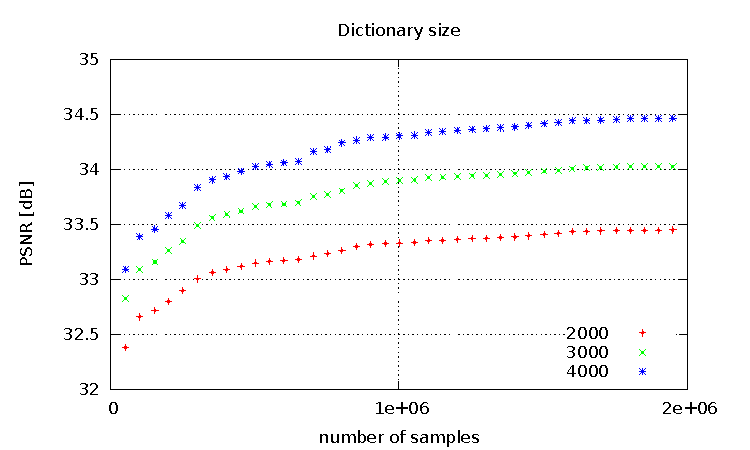
\includegraphics[width = 1.0\textwidth]{../tests/results/dictSizeLassoGod.pdf}
\caption{reconstruction quality for different dictionary sizes (Lasso)}
\label{fig:dictSizeGood}
\end{figure}

% We tried a diffrent strategy and addresed this issues with the clustering
% approach from \prettyref{sec:clustering}.
% \begin{figure}[h]
% \centering
% 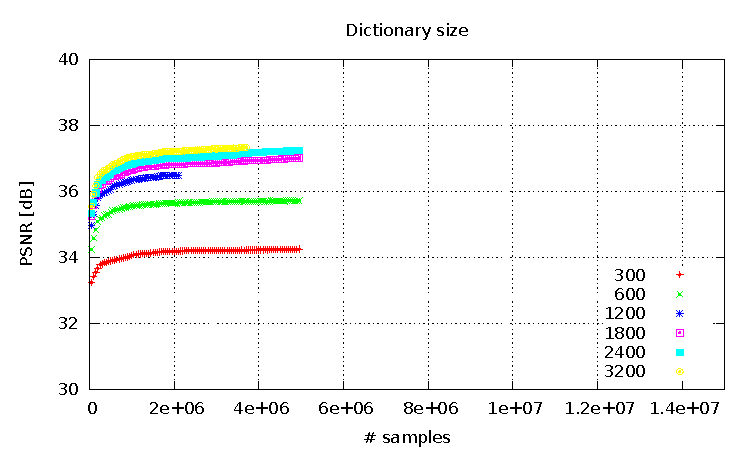
\includegraphics[width = 0.8\textwidth]{../tests/results/dictSizeOMP.pdf}
% \caption{reconstruction quality for different dictionary sizes (OMP)}
% \label{fig:dictSizeOMP}
% \end{figure}



\paragraph{Clustering}
We want to know if a dictionary merged from smaller dictionaries, learned in a
cluster, can lead to similar quality as a big dictionary learned on its own.

Learning with an average of 10 coefficients and a single dictionary of 4,000
elements are learned until convergence. And each of 10 clients in the cluster
learns a dictionary with 500 atoms from batches of 1,000 images. 

\prettyref{fig:coeffsConvergInc} shows reconstruction quality average for both
dictionaries.

% \begin{table}[h]
% \centering
% \begin{tabular}{| l | c | c |}
% \hline\hline
% Images & single & merged \\
% \hline
% inside & $34,29172 \pm 3,61$ & $35,04152 \pm 3,48$  \\
% outside & $35.5104 \pm 0.0$ & $35.5104 \pm 0.0$ \\
% \hline
% \end{tabular}
% \caption{single vs. cluster}
% \end{table}

\begin{figure}[H]
\centering
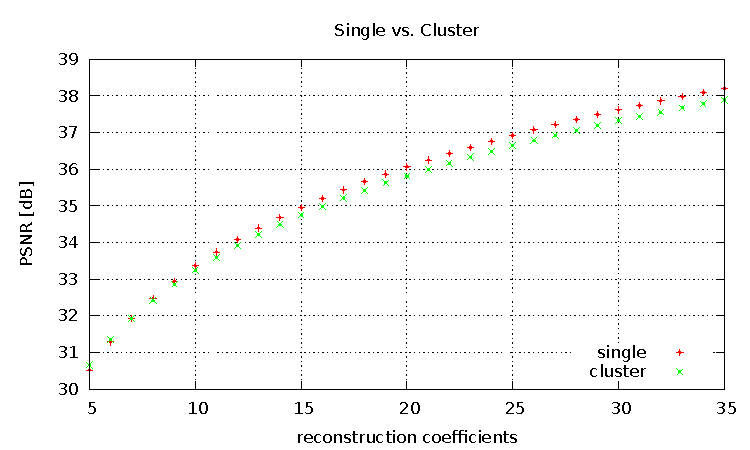
\includegraphics[width = 1.0\textwidth]{../tests/results/coeffsConvergInc.pdf}
\caption{reconstruction quality}
\label{fig:coeffsConvergInc}
\end{figure}

We see that the merged dictionary can reconstruct images with equal quality
as the big dictionary. And while convergence is not reaches yet we want to see
what we can already acomplish with the current dictionaries.


\clearpage
\section{Compression}
Besides the ability of learned dictionaries 
we use the simple compression algorithm from \prettyref{sec:compression}.
and compare it to a collection of JPEG and JPEG 2000 compressed images with the
same file size. Besides the raw pixel data, images formats usually contain a
certain amount of extra data from a file header and meta data. Fortunately we
can ignore this for simplification as the header data is only a few bytes and
large meta data was prevented during target compression. The selection of
images is limited as currently the process of obtaining the right settings for
the sparse coding compression are time consuming.
%and not being actual pixel data. 
The objective is to investigate the compression quality of our algorithm and
the dictionary and if the extra amount of index data is a big hit on the overall
load.

One benefit of the learned dictionary approach that plays well in our
hands is the ability to to learn and use specific dictionaries for each group of
images. We test this by learning a dictionary from a set of sketch images and
use it to compress sketches. A domain in which the JPEG compression performs
bad. As discovered before the natural images like block sizes of $8\times 8$
this is not necessarily true for the sketch images. They work fine with
$16\times 16$ blocks and enable us to reduce the amount of blocks.
\prettyref{fig:compressionDicts} shows the used dictionaries. 

The natural dictionary (\prettyref{fig:naturalDict}) consists of 4,000 $8 \times
8$ atoms merged from 100 sub dictionaries with 1,000 atoms. Each sub
dictionary was learned with 1,000 out of 100,000 images. Convergence of the
training process was already reached after 400 images. Taking less than 5
hours.

The sketch dictionary (\prettyref{fig:sketchDict}) consists of 1,000
$16\times 16$ atoms learned from 1,000 sketches.

\newpage
\begin{figure}[H]
\centering
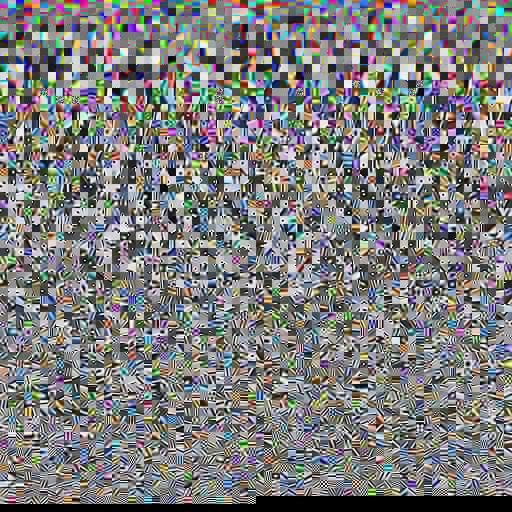
\includegraphics[width = 0.66\textwidth]{images/natural_dict.jpg}
\caption{Natural dictionary for compression}\label{fig:naturalDict}
\end{figure}
\begin{figure}[H]
\centering

\includegraphics[width = 0.66\textwidth]{images/sketch_dict.jpg}
\caption{Sketch dictionary for compression}\label{fig:sketchDict}
\end{figure}


\clearpage
\subsection{Results}
% Difference in the selection strategy.
% Very noisy vs. smooth. 
% How this different selection strategies affect the learning step will be
% presented in the next section.
\subsubsection{Natural images}

For the short time available the results are promising. Compression of
natural images can achieve similar quality as the JPEG algorithm
\prettyref{tab:compression1} for high compression rates but do not reach the
JPEG 2000 quality. Compression coding was done with the OMP as it turned out to
work better with the quantization step of our algorithm and requires less
coefficients. Looking at a lower compression ratio the results are much worse
than JPEG or JPEG2000. As the dictionaries have limited maximum reconstruction
quality.

\begin{table}[h]
%\caption{single vs. cluster}
\centering

\begin{tabular}{| l l | c | c | c|}
\hline\hline
Image & bpp & SPRS & JPEG & JPEG2000 \\
\hline
a & 1.12 & 31.2205 & 32.3289 & 36.6103 \\
%a & 1.12 & 31.2205 & 42.7488 &  \\
\hline
b & 1.01 & 34.7735 & 35.0671 & 40.3299 \\
%b & 1.01 & 34.7735 & 49.4725 & \\
\hline
c & 1.8  & 29.0597 & 27.2556 & 31.7412 \\
%c & 1.8  & 34.5818 & 40.8959 &  \\
\hline
d & 0.74 & 35.0531 & 35.5104 & 39.4195 \\
%d & 1.47  & 35.9499 & 42.3517 &  \\
\hline
e & 0.66 & 28.2658 & 32.0171 & 32.7864 \\
\hline
f & 1.53 & 24.6843  & 24.8492 & 26.2794 \\
\hline
\end{tabular}
\caption{natural image compression results}
\label{tab:compression1}.
\end{table} 

% \begin{figure}[h]
% \centering
% % \subfloat{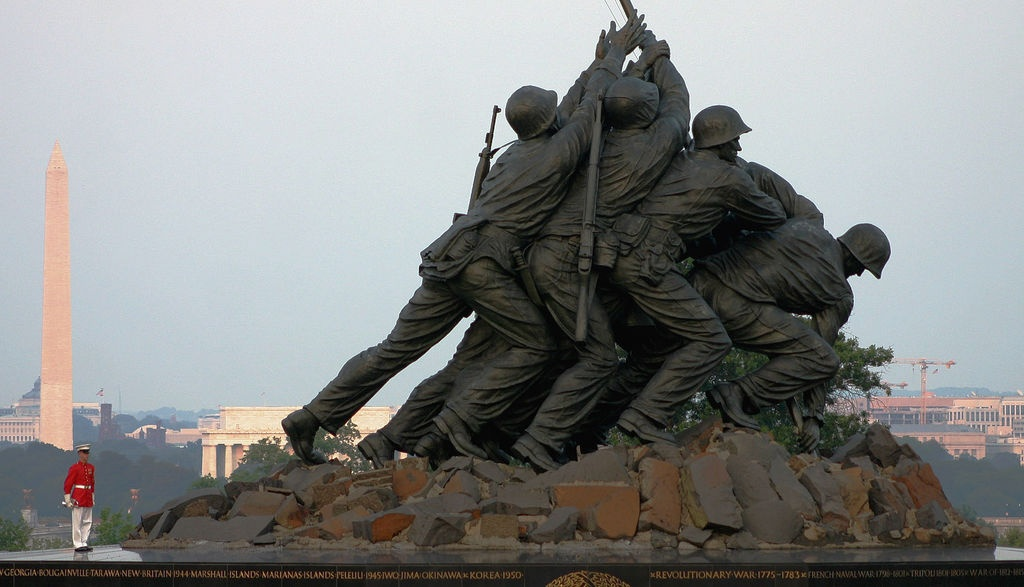
\includegraphics[width = 0.3\textwidth]{images/28979823.jpg}}
% % \hspace{5mm}
% % \subfloat{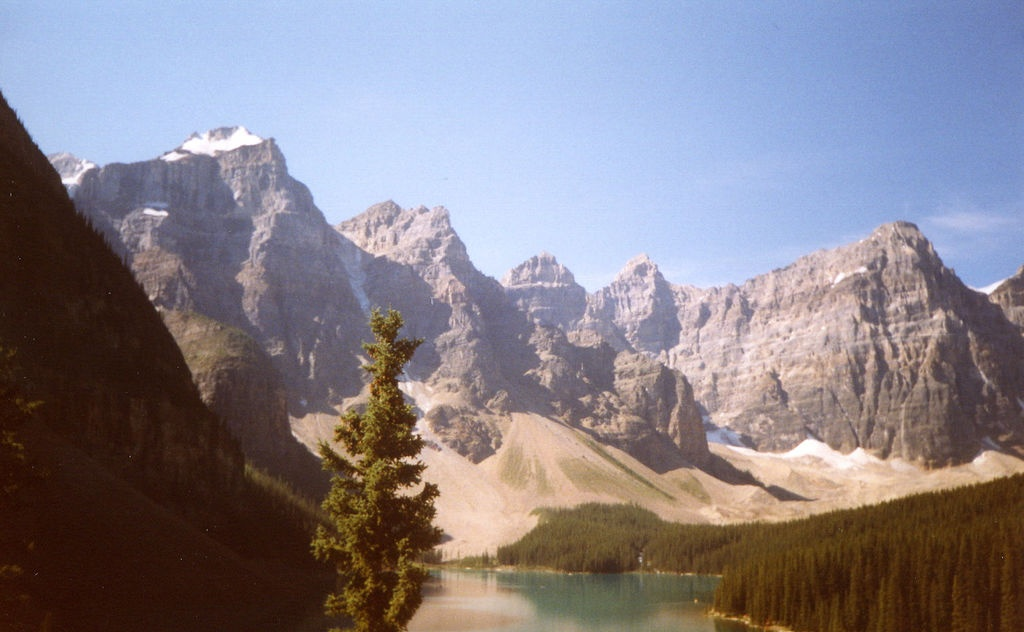
\includegraphics[width = 0.3\textwidth]{images/29018694.jpg}}
% % \hspace{5mm}
% \subfloat{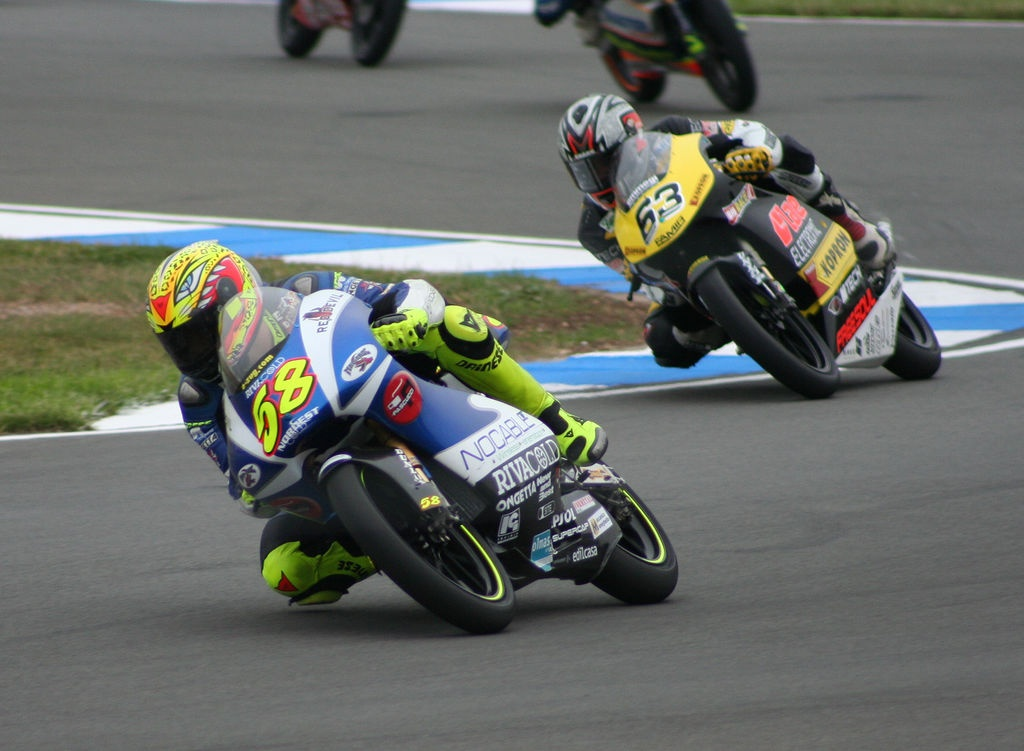
\includegraphics[width = 0.3\textwidth]{images/28803842.jpg}}
% \hspace{5mm}
% \subfloat{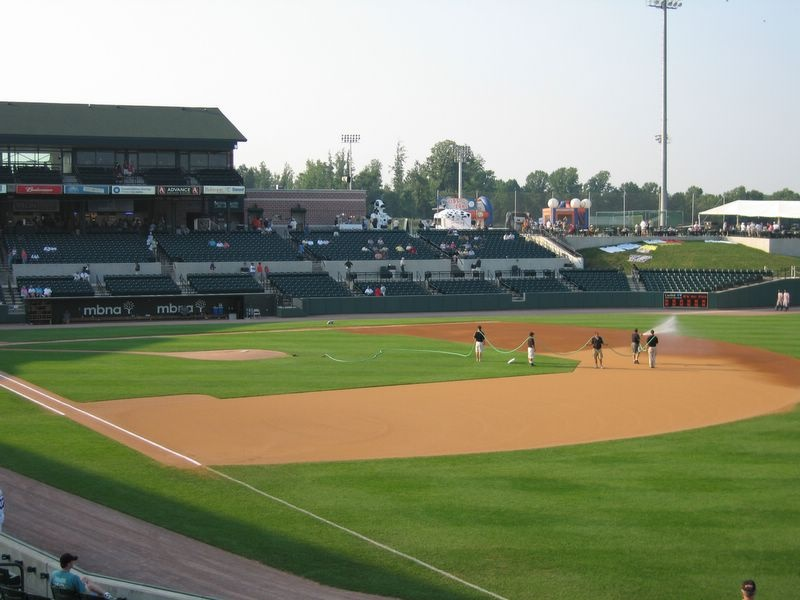
\includegraphics[width = 0.3\textwidth]{images/28894495.jpg}}
% \hspace{5mm}
% \subfloat{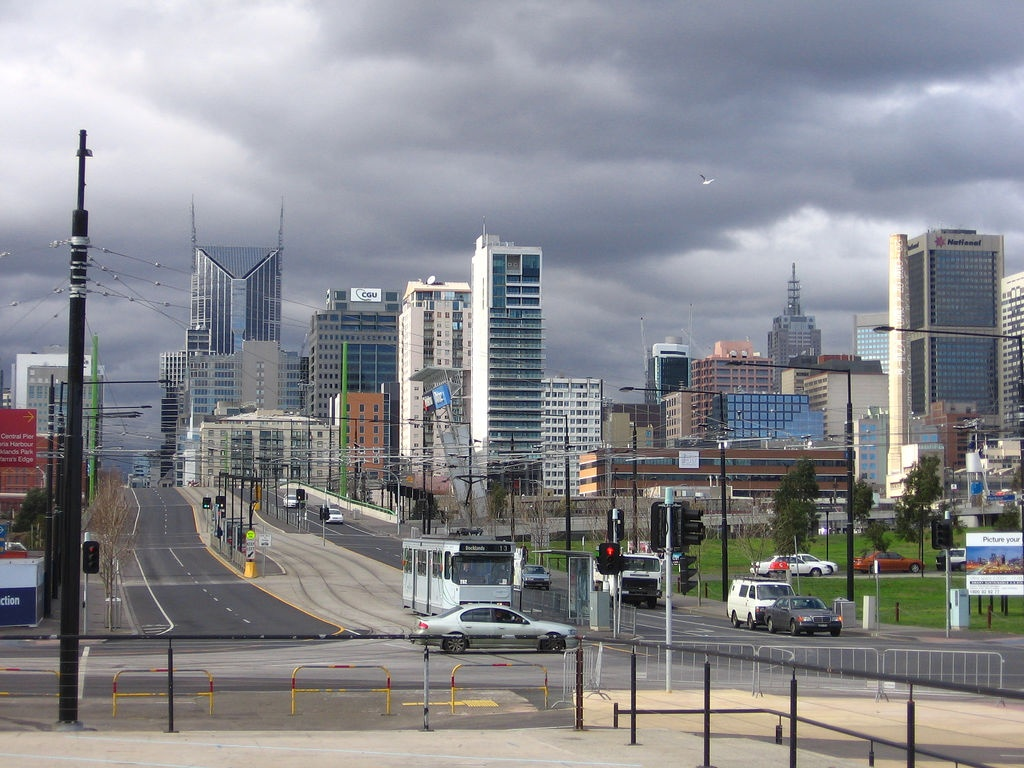
\includegraphics[width = 0.3\textwidth]{images/28952841.jpg}}
% \hspace{5mm}
% \subfloat{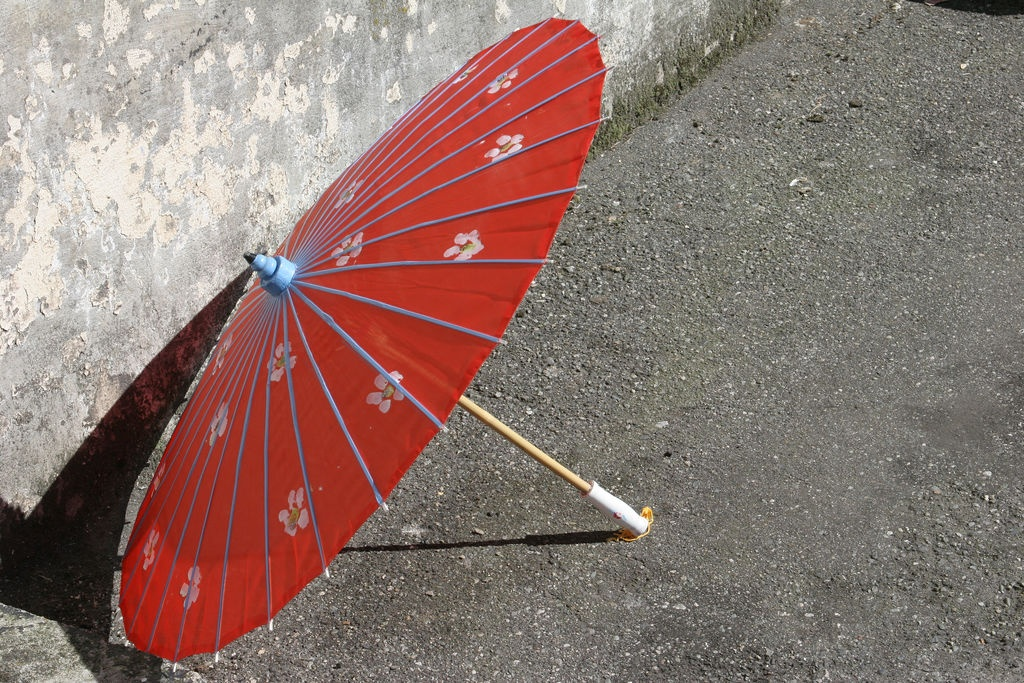
\includegraphics[width = 0.3\textwidth]{images/28874882.jpg}}
% \caption{natural images}
% %\label{fig:database_images}
% \end{figure}

\clearpage
\subsubsection{Sketches}
The high compression ratio results get even better when looking at the sketch
images (\prettyref{fig:sketches}). Our algorithm can surpasse the JPEG
compression (\prettyref{tab:compression2}) for low bit rates.
\prettyref{fig:magnified} show some magnified segments of image
\ref{fig:sketch3} to ilustrate the reconstruction features. There are less
artifacts than in the JPEG images. The line segment atoms from the dictionary
show similarities to the wavelet based JPEG 2000 compression.


\begin{table}[H]
%\caption{single vs. cluster}
\centering
\begin{tabular}{| c l | c | c | c|}
\hline\hline
Image & bpp & SPRS & JPEG & JPEG2000 \\
\hline
a & 0.084 & 33.9594 & 28.9578 & 38.3258  \\
%a & 0.084 & 33.9594 & 28.9578 & 38.3258  \\
\hline
b & 0.13 & 32.9002 & 34.5546 &  40.0159 \\
%b & 0.13 & 32.9002 & 34.5546 &  40.0159 \\
\hline
c & 0.08 & 32.5131 & 28.6558 & 36.3093  \\
%c & 0.08 & 32.5131 & 28.6558 & 36.3093  \\
\hline
\end{tabular}
\caption{sketch compression results}
\label{tab:compression2}
\end{table}
% \begin{figure}[h]
% \centering
% \setcounter{subfigure}{0}
% \subfloat[]{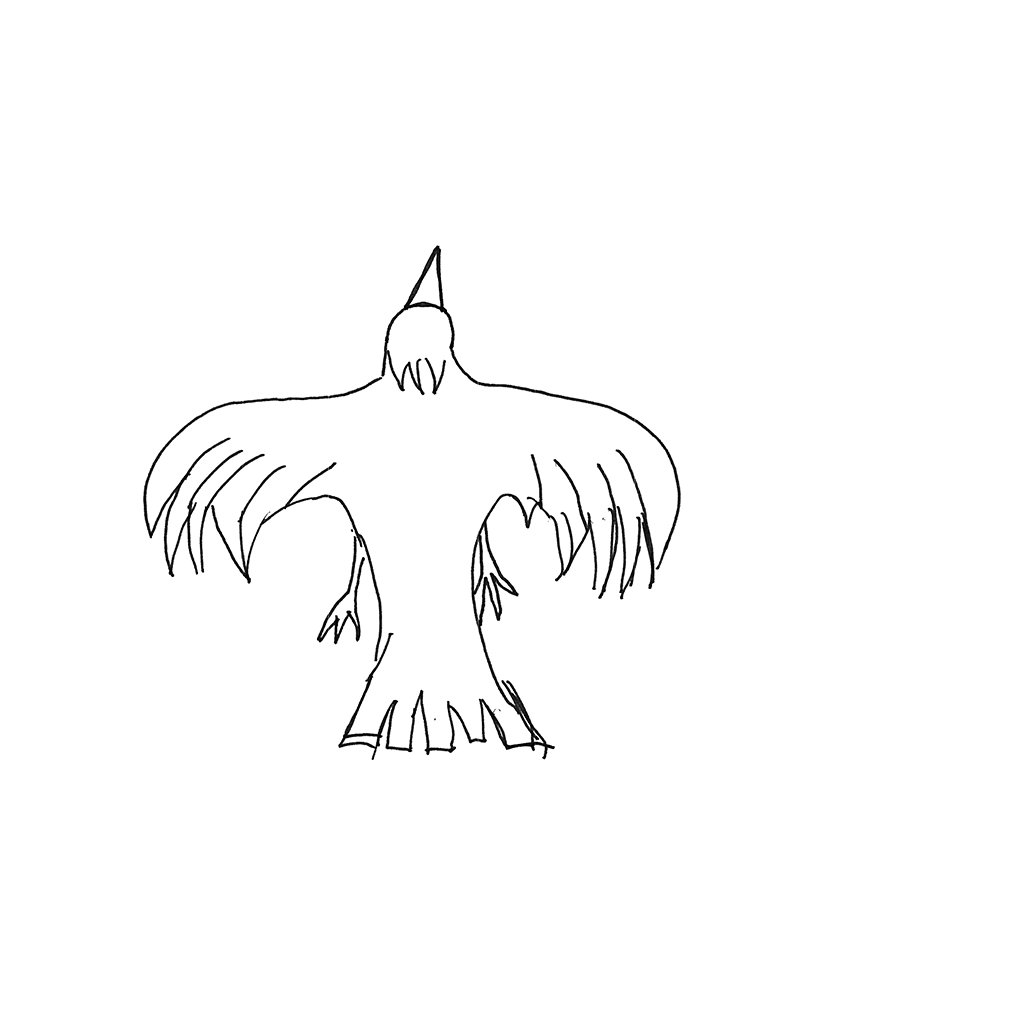
\includegraphics[width = 0.3\textwidth]{images/sketch1.jpg}}
% \hspace{5mm}
% \subfloat[]{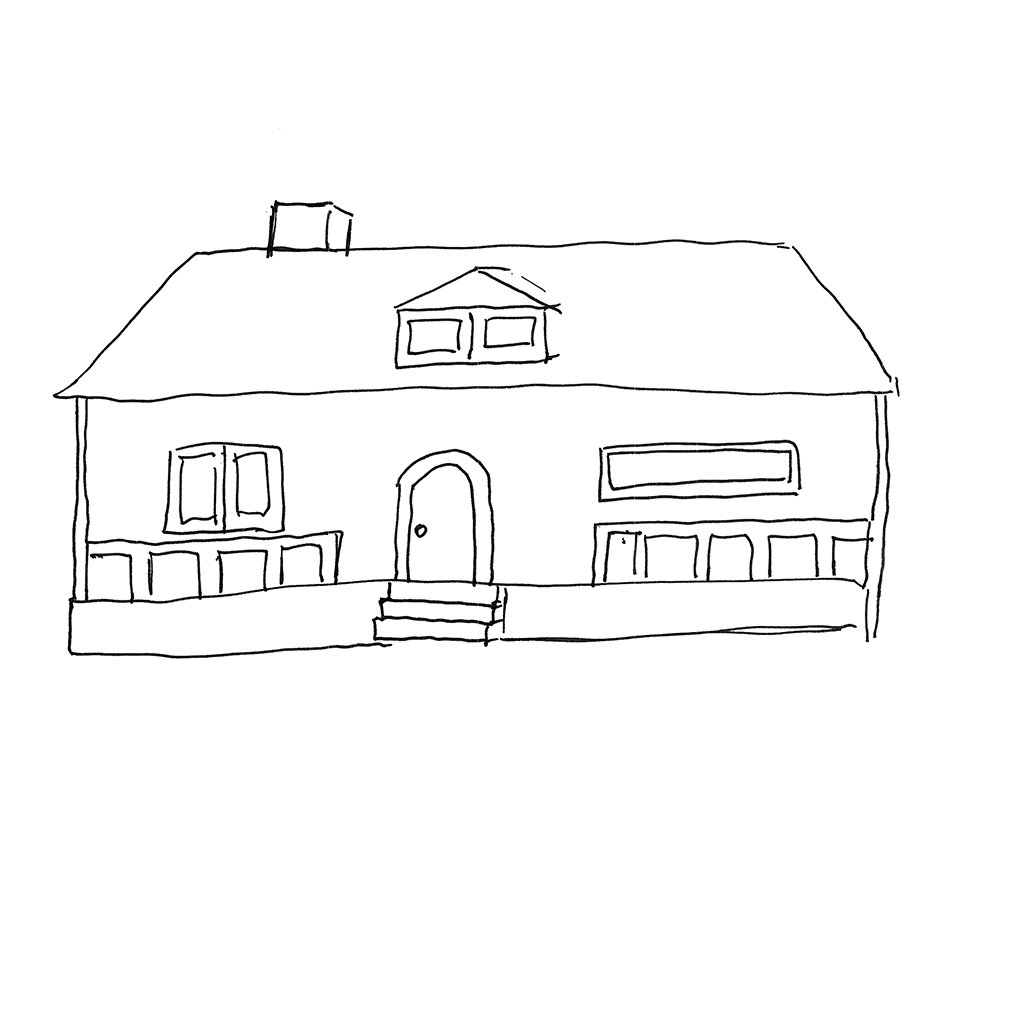
\includegraphics[width = 0.3\textwidth]{images/sketch2.jpg}}
% \hspace{5mm}
% \subfloat[]{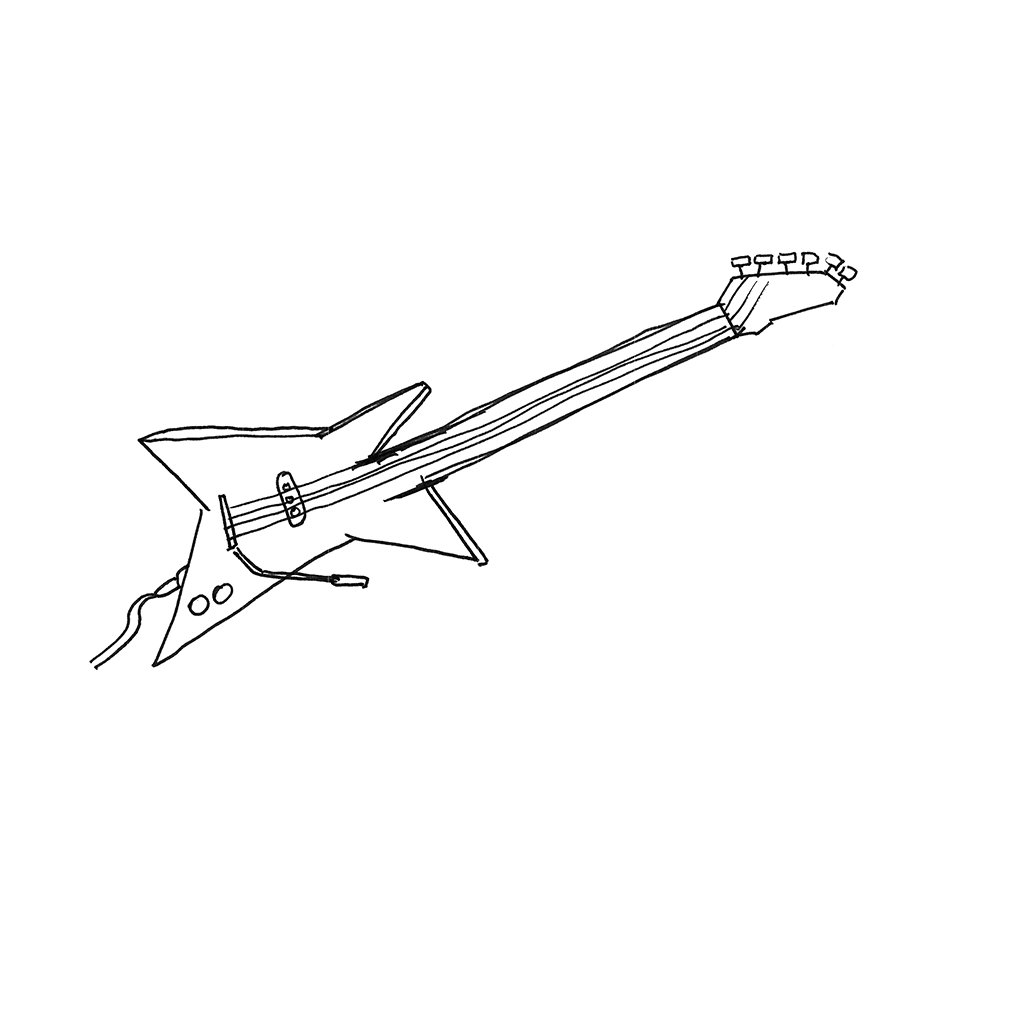
\includegraphics[width =
% 0.3\textwidth]{images/sketch3.jpg}\label{fig:sketch3}}
% \hspace{5mm}
% \caption{sketches}
% \label{fig:sketches}
% \end{figure}
%\newpage
\begin{figure}[h]
\centering
\subfloat[original]{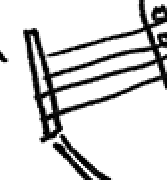
\includegraphics[width =
0.40\textwidth]{images/sketch_png_1.png}}
\hspace{5mm}
\subfloat[SPRS]{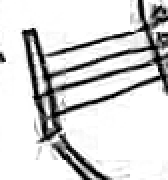
\includegraphics[width =
0.40\textwidth]{images/sketch_sprs_1.png}}
\hspace{25mm}
\subfloat[JPEG]{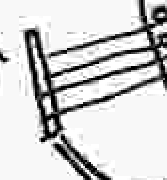
\includegraphics[width =
0.40\textwidth]{images/sketch_jpeg_1.png}}
\hspace{5mm}
\subfloat[JPEG2000]{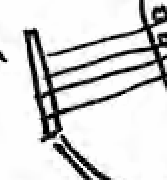
\includegraphics[width =
0.40\textwidth]{images/sketch_2000_1.png}}
\caption{}
\label{fig:magnified}
\end{figure}




















